\subsection{Question 1}

Nous pouvons construire le graphe de classes suivant :

\begin{figure}[H]
  \centering
  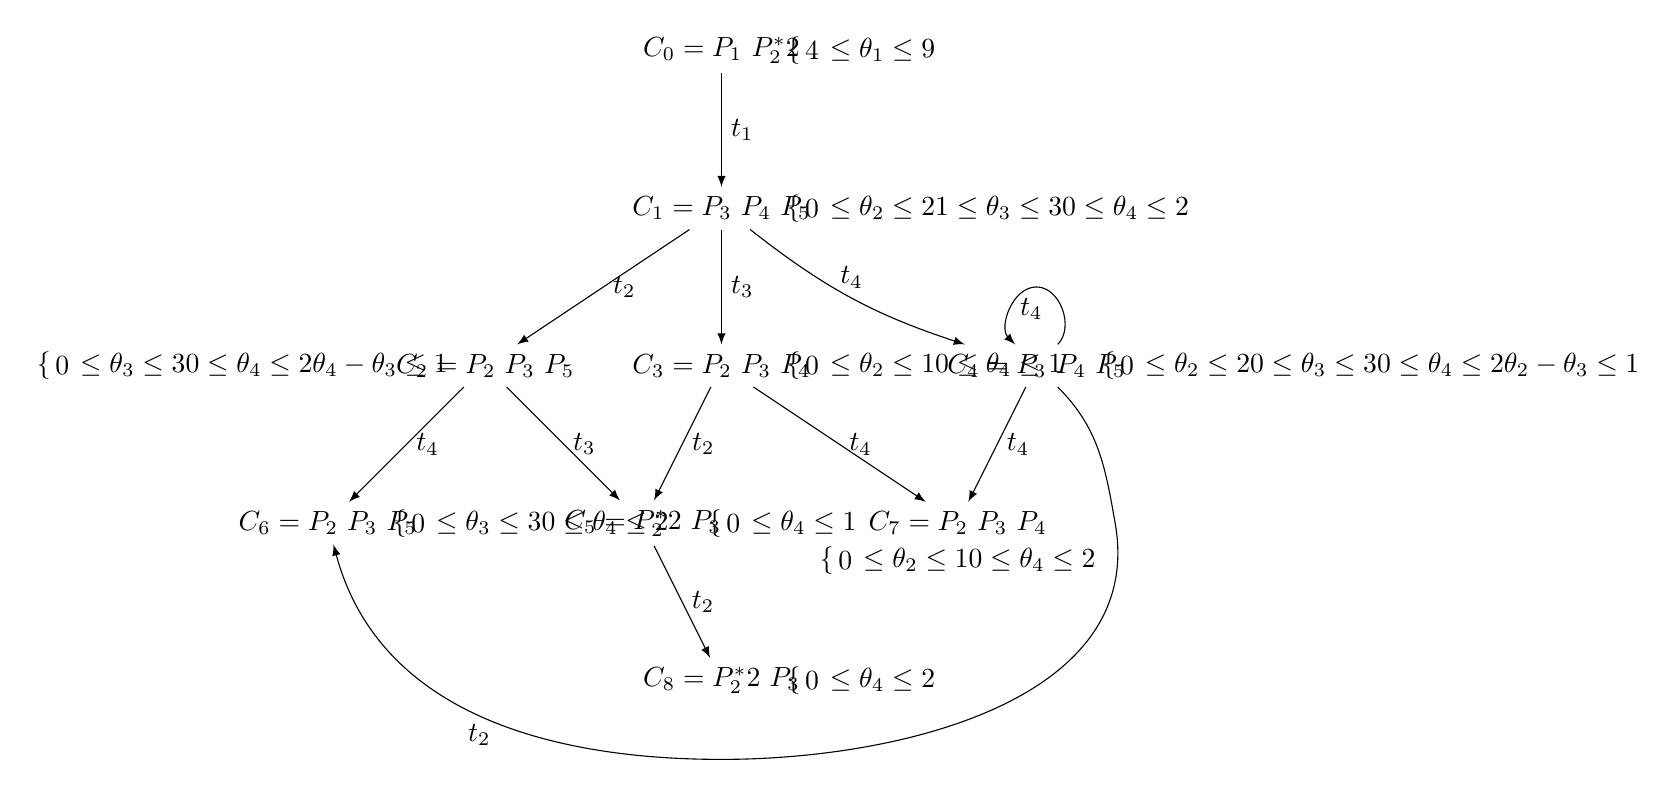
\begin{tikzpicture}
    % Liste des Marquages des classes
    \node (M0) at (0,8) {$C_0 = P_1\ P_2^*2$};
    \draw (0,8) node[right = 20pt] {$
      \begin{cases}
        4 \leq \theta_1 \leq 9
      \end{cases}
      $};
    \node (M1) at (0,6) {$C_1 = P_3\ P_4\ P_5$};
    \draw (0,6) node[right = 20pt] {$
      \begin{cases}
        0 \leq \theta_2 \leq 2\\
        1 \leq \theta_3 \leq 3\\
        0 \leq \theta_4 \leq 2
      \end{cases}
      $};
    \node (M2) at (-3,4) {$C_2 = P_2\ P_3\ P_5$};
    \draw (-3,4) node[left = 10pt] {$
      \begin{cases}
        0 \leq \theta_3 \leq 3\\
        0 \leq \theta_4 \leq 2\\
        \theta_4 - \theta_3 \leq 1
      \end{cases}
      $};
    \node (M3) at (0,4) {$C_3 = P_2\ P_3\ P_4$};
    \draw (0,4) node[right = 20pt] {$
      \begin{cases}
        0 \leq \theta_2 \leq 1\\
        0 \leq \theta_4 \leq 1
      \end{cases}
      $};
    \node (M4) at (4,4) {$C_4 = P_3\ P_4\ P_5$};
    \draw (4,4) node[right = 20pt] {$
      \begin{cases}
        0 \leq \theta_2 \leq 2\\
        0 \leq \theta_3 \leq 3\\
        0 \leq \theta_4 \leq 2\\
        \theta_2 - \theta_3 \leq 1
      \end{cases}
      $};
    \node (M5) at (-1,2) {$C_5 = P_2^*2\ P_3$};
    \draw (-1,2) node[right = 20pt] {$
      \begin{cases}
        0 \leq \theta_4 \leq 1
      \end{cases}
      $};
    \node (M6) at (-5,2) {$C_6 = P_2\ P_3\ P_5$};
    \draw (-5,2) node[right = 20pt] {$
      \begin{cases}
        0 \leq \theta_3 \leq 3\\
        0 \leq \theta_4 \leq 2
      \end{cases}
      $};
    \node (M7) at (3,2) {$C_7 = P_2\ P_3\ P_4$};
    \draw (3,2) node[below = 5pt] {$
      \begin{cases}
        0 \leq \theta_2 \leq 1\\
        0 \leq \theta_4 \leq 2
      \end{cases}
      $};
    \node (M8) at (0,0) {$C_8 = P_2^*2\ P_3$};
    \draw (0,0) node[right = 20pt] {$
      \begin{cases}
        0 \leq \theta_4 \leq 2
      \end{cases}
      $};



     % Liste des arcs
    \draw[->,>=latex] (M0) -- (M1) node[midway, right]{$t_1$};
    \draw[->,>=latex] (M1) -- (M2) node[midway, right]{$t_2$};
    \draw[->,>=latex] (M1) -- (M3) node[midway, right]{$t_3$};
    \draw[->,>=latex] (M1) to[bend right=10] node[midway, above]{$t_4$} (M4);
    \draw[->,>=latex] (M2) -- (M5) node[midway, right]{$t_3$};
    \draw[->,>=latex] (M2) -- (M6) node[midway, right]{$t_4$};
    \draw[->,>=latex] (M3) -- (M5) node[midway, right]{$t_2$};
    \draw[->,>=latex] (M3) -- (M7) node[midway, right]{$t_4$};
    \draw[->,>=latex] (M4) -- (M7) node[midway, right]{$t_4$};
    \draw[->,>=latex] (M5) -- (M8) node[midway, right]{$t_2$};
    \draw[->,>=latex] (M4) to[out=45, in=0] (4,5) to[out=180, in=135] node[midway, right]{$t_4$} (M4);
    \draw[->,>=latex] (M4) to[out=-45,in=100] (5,2)to[out=-80, in=0] (0,-1) to[out=180, in=-75] node[midway, below]{$t_2$} (M6);


  \end{tikzpicture}
  \caption{Graphe des classes} \label{fig:M10}
\end{figure}


\subsection{Question 2}

Dans ce graphe des classes nous n'avons que des composantes fortement connexe unitaire.

\begin{figure}[H]
  \centering
  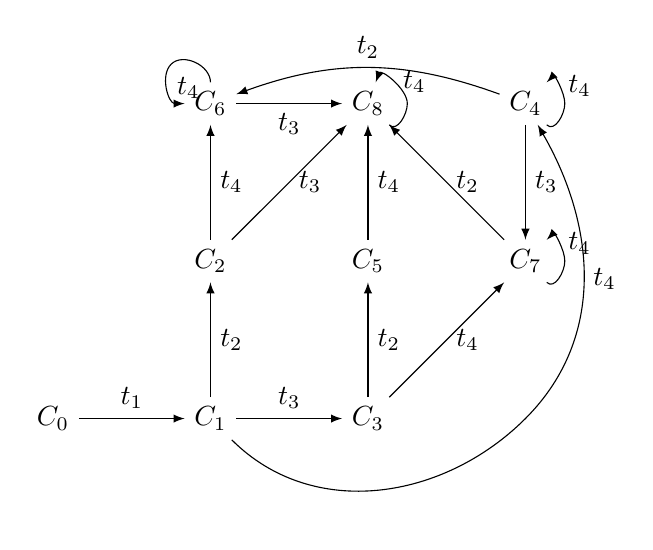
\begin{tikzpicture}
    % Liste des Marquages des classes
    \node (C0) at (0,0) {$C_0$};
    \node (C1) at (2,0) {$C_1$};
    \node (C2) at (2,2) {$C_2$};
    \node (C3) at (4,0) {$C_3$};
    \node (C4) at (6,4) {$C_4$};
    \node (C5) at (4,2) {$C_5$};
    \node (C6) at (2,4) {$C_6$};
    \node (C7) at (6,2) {$C_7$};
    \node (C8) at (4,4) {$C_8$};

 % Liste des arcs
    \draw[->,>=latex] (C0) -- (C1) node[midway, above]{$t_1$};
    \draw[->,>=latex] (C1) -- (C2) node[midway, right]{$t_2$};
    \draw[->,>=latex] (C1) -- (C3) node[midway, above]{$t_3$};
    \draw[->,>=latex] (C2) -- (C6) node[midway, right]{$t_4$};
    \draw[->,>=latex] (C2) -- (C8) node[midway, right]{$t_3$};
    \draw[->,>=latex] (C3) -- (C5) node[midway, right]{$t_2$};
    \draw[->,>=latex] (C3) -- (C7) node[midway, right]{$t_4$};
    \draw[->,>=latex] (C6) -- (C8) node[midway, below]{$t_3$};
    \draw[->,>=latex] (C5) -- (C8) node[midway, right]{$t_4$};
    \draw[->,>=latex] (C7) -- (C8) node[midway, right]{$t_2$};
    \draw[->,>=latex] (C4) -- (C7) node[midway, right]{$t_3$};
    \draw[->,>=latex] (C4) to[bend right=20] node[midway, above]{$t_2$} (C6);
    \draw[->,>=latex] (C1) to[out=-45, in=225] (6,0) to[out=45, in=-60] node[midway, right]{$t_4$}(C4);
    \draw[->,>=latex] (C6) to[out=90, in=45] (1.5,4.5) to[out=225, in=180] node[midway, right]{$t_4$}(C6);
    \draw[->,>=latex] (C8) to[out=-45, in=-90] (4.5,4) to[out=90, in=70] node[midway, right]{$t_4$}(C8);
    \draw[->,>=latex] (C4) to[out=-45, in=-90] (6.5,4) to[out=90, in=45] node[midway, right]{$t_4$}(C4);
    \draw[->,>=latex] (C7) to[out=-45, in=-90] (6.5,2) to[out=90, in=45] node[midway, right]{$t_4$}(C7);


  \end{tikzpicture}
  \caption{Graphe des composantes fortement connexes} \label{fig:M10}
\end{figure}
